\chapter{Discussion}
\label{cha:Discussion}

The overall performance of the models compares well to the scoring functions introduced in \cite[]{Birklbauer2021}.
The following table represents the results for the \acrshort*[]{ache} protein in \cite[]{Birklbauer2021}:
\begin{figure}[H]
    \begin{center}
        \caption[]{Scoring results for ACHE Birklbauer}
        \label{fig:ache_birklbauer}
        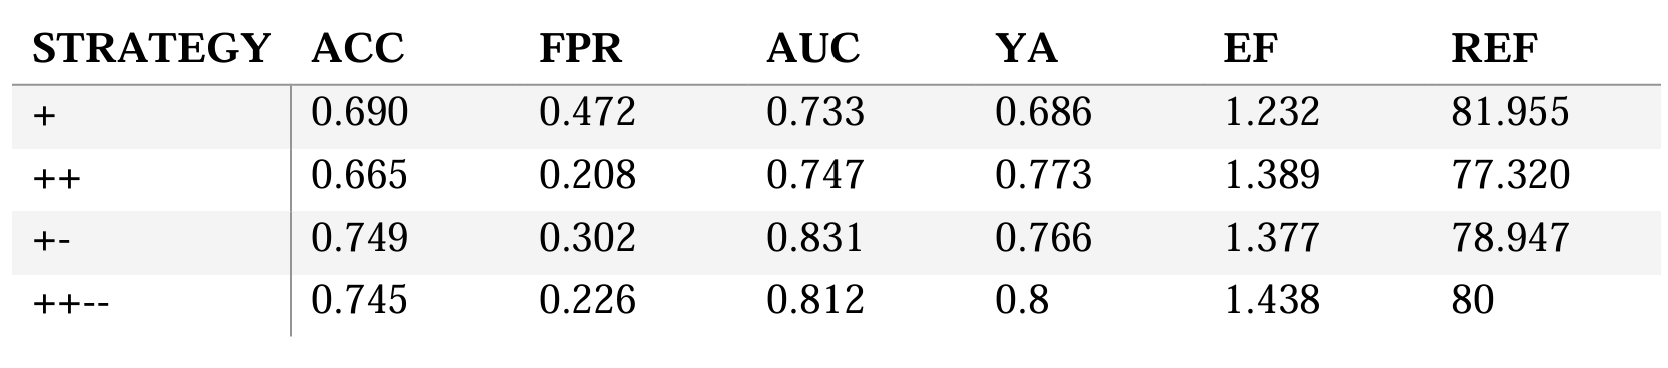
\includegraphics[width=14cm]{discussion/Birklbauer_ACHE.png}
    \end{center}
\end{figure}
The following results were achieved for the \acrshort*[]{ache} protein using the methods proposed in this thesis:
\begin{table}[H]
    \begin{center}
        \caption{Acetylcholinesterase performance test-set}
        \begin{tabular}{lrrrrrr}
            \toprule
            Name             & ACC    & FPR    & AUC    & YA     & EF     & REF     \\
            \midrule
            baseline\_rf     & 0.8106 & 0.3285 & 0.7992 & 0.7716 & 1.4161 & 92.6829 \\
            fe\_smote\_rf    & 0.8007 & 0.3358 & 0.7894 & 0.7653 & 1.4046 & 91.4634 \\
            fe\_smote\_nn    & 0.7708 & 0.2993 & 0.7650 & 0.7684 & 1.4102 & 82.9268 \\
            baseline\_nn     & 0.7674 & 0.2920 & 0.7626 & 0.7701 & 1.4134 & 81.7073 \\
            fe\_rf\_per\_knn & 0.7575 & 0.4307 & 0.7420 & 0.7177 & 1.3172 & 91.4634 \\
            baseline\_knn    & 0.6844 & 0.5766 & 0.6629 & 0.6520 & 1.1966 & 90.2439 \\
            fe\_rf\_mdi\_knn & 0.5515 & 0.4307 & 0.5530 & 0.5986 & 1.0987 & 59.8639 \\
            \bottomrule
        \end{tabular}
    \end{center}
\end{table}

The comparison between the two tables underlines the performance improvements of the machine learning approaches
over the simple scoring functions introduced in \cite[]{Birklbauer2021}.
Generally the improvements in \acrshort*[]{acc} and \acrshort*[]{ref} are most notable.
The improvements in the \acrshort*[]{ref} metric are of particular interest, as there is less money spent on investigating false positive compounds.
Similar performance benefits can be observed for the other protein complexes.

\section{Improvements and outlook}
This thesis serves as a proof of concept for the applicability of machine learning models in combination with feature engineering for protein docking, as the achieved results 
are more accurate than those achieved using traditional approaches.

However, the machine learning approaches for protein docking where implemented using standard approaches and models. 
Through the use of more problem-tailored algorithmic methods the quality of the results will probably increase. Additionally, only a small sample 
of protein-ligand complexes was researched for this thesis. The machine learning methods proposed within this thesis need to be evaluated on a larger subset of 
protein-ligand compounds to determine whether machine learning is a viable approach for protein docking.
